\documentclass[12pt,letterpaper]{article}

\usepackage{amsmath, amsthm}
\usepackage{graphicx}
\usepackage{microtype, parskip}
\usepackage{caption, subcaption, multirow, morefloats, rotating, longtable}
\usepackage{hyperref}
\usepackage[numbers,sort&compress]{natbib}
\usepackage{authblk, attrib, fullpage}
\usepackage{lineno}


\begin{document}
\setcounter{secnumdepth}{0}

\begin{titlepage}
  \begin{center}
    \huge{Evolutionary paleoecology and the biology of extinction}

    \vspace{1.5cm}

    \large{Peter D. Smits \\}
    \footnotesize{\href{mailto:psmits@uchicago.edu}{psmits@uchicago.edu}}

    \vspace{1.5cm}

    Dissertation Proposal Hearing \\
    \today \\
    Commmittee on Evolutionary Biology \\
    The University of Chicago

    \vspace{1.5cm}

    \textit{Committee} \\
    Dr. Michael J. Foote (co-advisor) \\
    Dr. Kenneth D. Angielczyk (co-advisor) \\
    Dr. Richard H. Ree \\
    Dr. P. David Polly
  \end{center}
\end{titlepage}

\linenumbers
\modulolinenumbers[2]


\section{Introduction and Theory}
%Paleobiology is the study of life over time and the inference of what processes generate the observed patterns in diversity and disparity. Intimately related to paleobiology is the concept of macroevolution here defined as the pattern of speciation and extinction over time \citep{Jablonski2008a}. The study of macroevolution is the estimation of the processes underlying these observed patterns. The term origination is frequently used in place of speciation because it includes both speciation and migration and depending on both the spatial scale and quality of the fossil record it may be impossible to distinguish between the two.
%
Evolutionary paleoecology is the study of the effects of ecological traits and factors on differential rate dynamics, particularly rates of faunal turnover and diversification \citep{Kitchell1985a}. Ecological traits and factors are traits expressed by a taxon, at any level, that are involved with biotic--biotic or biotic--abiotic interactions. Diversification is the difference between origination and extinction and is the net pattern of macroevolution. The study of evolutionary paleoecology is therefore the link between environmental (biotic--biotic and biotic--abiotic) interactions and macroevolution. As a corollary to \citet{Kitchell1985a}'s definition, \citet{Allmon1994} states that in order to correctly link ecological interactions to macroevolution, one must focus on the specific traits and factors that may affect the speciation process. Tacitly included in this is the study of how ecological traits are related to extinction \citep{Kitchell1990}.

Geographic range size is considered one of the best understood species level traits \citep{Jablonski2008a}, and there is a strong relationship between geographic range size and extinction risk. Species with larger geographic ranges tend to have lower extinction rates than species with smaller geographic ranges \citep{Jablonski1986,Harnik2013,Nurnberg2013a,Jablonski2003,Roy2009c}. Range size is considered emergent because no one property of an organism can explain this trait and instead is the combination of multiple properties. The effects of various organismal traits, such as those relating to environmental preference, together or in concert remain less understood. Ecological traits have been shown to be related to differential extinction \citep{Foote2013,Liow2007b,Baumiller1993,Nurnberg2013a}, especially the relationship of adaptation to variable environments and increased species longevity. While some research has focused on the indirect effect of organismal traits on longevity \citep{Harnik2011}, the additive or interactive effects of organismal traits and their relationship to survival remain understudied. Here I propose to study the how organismal traits related to range size and if emergent traits are necessary for best explaining extinction.

Survival can be considered the fundamental measure evolutionary success because ultimately, a successful lineage is not one that speciated greatly but one that never went extinct \citep{Cooper1984,Palmer2012}. Because during periods of background extinction, extinction is most likely non-random with respect to biology \citep{Jablonski1986}, it should be possible to estimate how various ecological traits are correlated with survival \citep{Kitchell1990,Kitchell1985a}. Periods of background extinction also represent the majority of geologic time and remain relatively predictable and change slowly, providing a better opportunity to study how traits are related to survival than during mass extinctions \citep{Jablonski1986,Raup1988}. Additionally, the Law of Constant extinction \citep{VanValen1973} states that extinction rate within an adaptive zone is taxon-age independent. By analyzing the survival patterns within different adaptive zones during periods of background extinction, it should be possible to determine if extinction is best modeled as age independent or dependent (accelerating/decelerating).

It is under this framework that I propose to study how ecological traits associated with environmental preference and adaptive zone have affected the differential survival and cosmopolitan-endemism dynamics. I will be studying two distantly related and biotically different groups: Permian brachiopods and Cenozoic mammals. Both of these groups are considered to have very good fossil records able to reflect massive long term evolutionary patterns \citep{Mark1977}. These two time periods were chosen because they represent periods of approximately the same length (47 My and 65 My) and of climatic change, global warming and global cooling respectively. Also, these two groups are a marine and terrestrial system respectively and the traits associated with range size and environmental preference (described below) are fundamentally very different. 

Importantly, these two groups allow for a hierarchy of questions to be asked. Both the brachiopod and mammal survival can be analyzed at the generic level and for different adaptive zones (combinations of traits). The age independence or dependence of extinction for these two groups can then be tested. However because there is a known biasing factor towards age-dependent extinction when analyzing generic level survival curves \citep{Simpson2006,Raup1978,Raup1991a}, the mammalian survival will be further analyzed at the specific level and the differences between the two survival functions will be examined, specifically in whether different traits best model the two curves and if either is age-independent or not. Additionally, the importance of global climatic change in modeling mammalian survival will be analyzed. If global climatic change is found to not be important for modeling mammalian survival this does not, however, mean that regional or local climatic changes are not important for modeling survival patterns. By analyzing mammalian community connectedness, it should then be possible to estimate how disjoint communities are and if it is reasonable expect global, regional, or local processes to dominate and if this changes over time.


\section{Permian brachiopods, extinction and environmental preference}

\textit{Questions:} In Australasian Permian brachiopods, do traits directly related to environmental preference relate to differential survival? Are certain traits more explanatory of survival than others? Does changing climate, habitat or substrate availability affect survival?

\textit{Background and Predictions:}
In brachiopods, three important ecological traits potentially involved in determining environmental preference are affixing strategy, substrate preference, and habitat preference. While larval mode is considered important in determining range size in marine invertebrates \citep{Jablonski2006a,Jablonski1983}, this does not preserve in brachiopods and thus cannot be used to directly model survivorship \citep{Jablonski1983}. Substrate preference is related to the chemical and physical processes affecting an environment and may limit the range of possible environments in which an organism can optimally survive. This then limits the possible geographic extent of a taxon. Substrate selection is mitigated via larval chemosensory abilities and thus may be a weak proxy for larval dispersal ability \citep{Jablonski2006a,Jablonski1983}. 

Affixing strategy and habitat preference relate to range size by limiting the possible geographic extent of a taxon. Affixing strategy is the manner by with an individual interfaces with the substrate and different strategies are optimal for different environmental conditions such as flow speed or mud depth \citep{Alexander1977,LaBarbera1978,LaBarbera1981}. Because brachiopods are obligate filter feeders, environmental energetics is important for prey capture and individual survival. Thus, the availability of optimal environments becomes a limiting factor on the possible geographic extent of a taxon. Habitat preference is a statement of the suitability of an environment and the accompanying environmental energy level and acts as a limit on the possible geographic extent of a taxon. 

The three principle ways of classifying affixing strategies are pedunculate, reclining, and cementing. During the Permian, pedunculate taxa tend to be associated with shallow on-shore environments while reclining taxa are associated with deep off-shore environments \citep{Clapham2007}. However, this association is weak as most assemblages are composed of a heterogeneous mix of taxa \citep{Clapham2007}. Previous analysis of brachiopod durations showed that affixing strategy is correlated with longevity \citep{Alexander1977} and that among endemic taxa reclining taxa had longer durations than other affixing strategies. In contrast, among cosmopolitan taxa pedunculate and cementing taxa had longer durations than all other taxa. However, if affixing strategy is not important for best modeling survival, than this may indicate that either the environmental energetics of the Australasia was rather uniform or that other factors were more important for determining survival. This would mean that while affixing strategy might be correlated with differential survival, it may only be a minor factor compared other environmental properties.

The three principle classifications of substrate affinity are carbonate, clastic, or mixed. These are descriptions of the lithology of the sites at which the taxa are predominately found \citep{Foote2006,Anderson2011a,Nurnberg2013a,Kiessling2007a,Miller2001}. The Pharenozoic is characterized by an overall decline in carbonates relative to clastics \citep{Foote2006,Miller2001}. Because of this, it is expected that taxa with clasitic or mixed affinities will have greater durations than taxa associated with carbonate substrates. If substrate affinity is found to have no importance for modeling survival, than this may mean that depositional environment has little to no affect on survival and that other factors relating to the environment, both measured and unmeasured, might dominate. Additionally, if substrate affinity is not found important for modeling survival, this may mean that depositional environments were relatively constant throughout the Permian of Australasia.

The primary ways of classifying habitat preference are on-shore, off-shore, or mixed. Habitat preference has been the focus of a great deal of research in terms of explaining global diversity dynamics \citep{Sepkoski1991,Kiessling2007a,Bottjer1988,Jablonski1991,Jablonski1983b}. Importantly, habitat preference is related to sea-level rise and fall and the availability of that habitat with changing environment. On-shore environments have declined in areal extent over the Pharenozoic \citep{Peters2008}. Because of this decrease in areal extent, the expectation would be that taxa predominately associated with on-shore habitats would have overall lower durations than taxa associated with off-shore habitats or mixed preference. If environmental preference is found to be unimportant when modeling brachiopod survival, this may mean that sea-level dynamics are rather constant through out Australasia or that other factors, both measured and unmeasured, may have dominated.

An important consideration is that taxonomic survival might not be linked to single environments \textit{per se}, but the variability of environments \citep{Foote2013,Heim2011,Liow2007b}. This adaptation to variable environments has been found to relate strongly with survival past origination \citep{Foote2013}. In this case, it would be expected then that taxa with mixed preferences for both substrate and habitat would have potentially longer durations than taxa with single preferences. This makes logical sense as it would mean that a taxon's potential geographic extent is not expressly limited by either of these two traits and thus decreasing expected extinction rate due to large range size \citep{Jablonski1986,Harnik2013,Nurnberg2013a,Jablonski2003,Roy2009c}. 

During the Permian there was a shift from an ``ice house'' to a ``hot house'' world \citep{Fielding2006,Birgenheier2010,Jones2006,Powell2007} which could be expected to have some effect on brachiopod survivorship. Taxa in Australia are of particular interest because of their proximity to the south pole during the Permian and the repeated glacial activity in the region \citep{Fielding2006,Birgenheier2010,Jones2006}. According to \citet{Olszewski2004}, sea-level and climate change do not wholly explain the ecological dynamics experienced by brachiopods in the Permian of Texas. The prediction then is that the best model of brachiopod survivorship will have to have some biotic component such as affixing strategy or substrate preference. Climate being a predictor in the best model of survivorship is less clear cut and necessary to determine empirically.


\textit{Proposed research:}
I propose to a survival analysis approach to compare the patterns of survivorship in Permian brachiopods. Survival analysis is the analysis of time-till-event data. In a paleontological context this is the time from origination (first appearance date; FAD) till extinction (last appearance date; LAD). I restrict this analysis to Australiasia because it represents a relatively continually sampled and well worked area that preserves the majority of the entire Permian \citep{Clapham2012,Clapham2008a,Waterhouse1987,Archbold1995}. Multiple models of survival with various combinations, both additive and interactive, of the organismal traits described above will be compared. Substrate preference, affixing strategy, and habitat perference will be assumed to be constant for the duration of the taxon and modeled as time-independent covariates. Because climate is known to change over time, it will be modeled as either an ancillary Heaviside function or a time-dependent covariate.

Because substrate and habitat occurrences are not constant at the species level, it is necessary to determine the most probable of assignments. The lithology of all occurrences will be classified into one of the three substrate affinity categories following \citet{Foote2006} while paleoenvironmental setting of all occurrences will be classified into one of the three habitat preferences following \citet{Kiessling2007}. Both of these traits will be assigned to all taxa following \citet{Simpson2009} where trait value are determined as the posterior probability of a taxon's occurrences in comparison to available options during the duration of said taxon. Assignment probability (\(P(H_{1}|E)\)) will be calculated as
\begin{equation}
  P(H_{1}|E) = \frac{P(E|H_{1})P(H_{1})}{P(E|H_{1})P(H_{1}) + P(E|H_{2})P(H_{2})}
  \label{eq:aff}
\end{equation}
where \(P(H_{1})\) and \(P(H_{2})\) are the prior probabilities of assignment while \(P(E|H_{1})\) and \(P(E|H_{2})\) are conditional, binomial probabilities. 

In order to asses if the best model of survival is age independent or dependent, the distribution of survival will be modeled using various different probability distributions (i.e. exponential, Weibull, log-normal, etc.). An exponential distribution represents the Law of Constant extinction as the rate parameter (\(\lambda\)) is constant with respect to time. In contrast, the Weibull distribution has two parameters, scale (\(\lambda\)) and shape (\(k\)). The scale parameter analogous to the \(\lambda\) of the exponential distribution while the shape parameter describes whether \(\lambda\) is accelerating (\(k < 1\)), decelerating (\(k > 1\)), or constant (\(k = 1\)) such as in the case of the exponential distribution.

Permian brachiopod occurrence information is available via the Paleobiology Database (PBDB; \url{http://fossilworks.org}) and is primarily based on the work of Clapham \citep{Clapham2006,Clapham2008a,Clapham2007a,Clapham2012,Clapham2007} and \citet{Waterhouse1987}.


\textit{Preliminary results}
Preliminary analysis of brachiopod survivorship was restricted to taxa that originated within the Permian. Survival was compared analyzed using substrate affinity and habitat preference. For substrate affinity, the priors of Eq. \ref{eq:aff} were \(P(H_{1}) = P(H_{2}) = 0.5\) and if \(P(H_{1}|E) > \frac{2}{3}\) then the taxon was considered of carbonate affinity while if \(P(H_{1}|E) < \frac{1}{3}\) then the taxon was considered to have a clastic affinity. Otherwise, the taxon was considered to have no or mixed affinity. In the case of habitat affinity, the posterior probability for each habitat (inshore, offshore, none) was calculated using Eq. \ref{eq:aff} with priors of \(P(H_{1}) = \frac{1}{3}\) and \(P(H_{2}) = \frac{2}{3}\) and the preference with maximum of the three posterior probabilities was the assignment.

Preliminary model fitting with both exponential and Weibull hazard functions and either or both trait indicated that the best fit model, based on comparison of AICc scores \citep{Hurvich1989,Akaike1974,Burnham2002a}, was the model with substrate affinity as the sole predictor and a Weibull hazard function. This model is illustrated below (Fig. \ref{subfig:aff_surv}). While this is the preliminarily best model of survivorship, the model with both substrate affinity and habitat preference as additive effects and a Weibull hazard function can be also considered a good model of survival (\(\Delta\)AICc \(\approx 2.9\)). Additionally, as illustrated by the difference between the nonparametric Kaplan--Meier survival curves and the predictions of the parametric model of survival (Fig. \ref{subfig:aff_surv}) and there is room for improvement in model specification.

\begin{figure}[ht]
%  \begin{center}
    \begin{subfigure}[b]{0.5\textwidth}
      \caption{}
      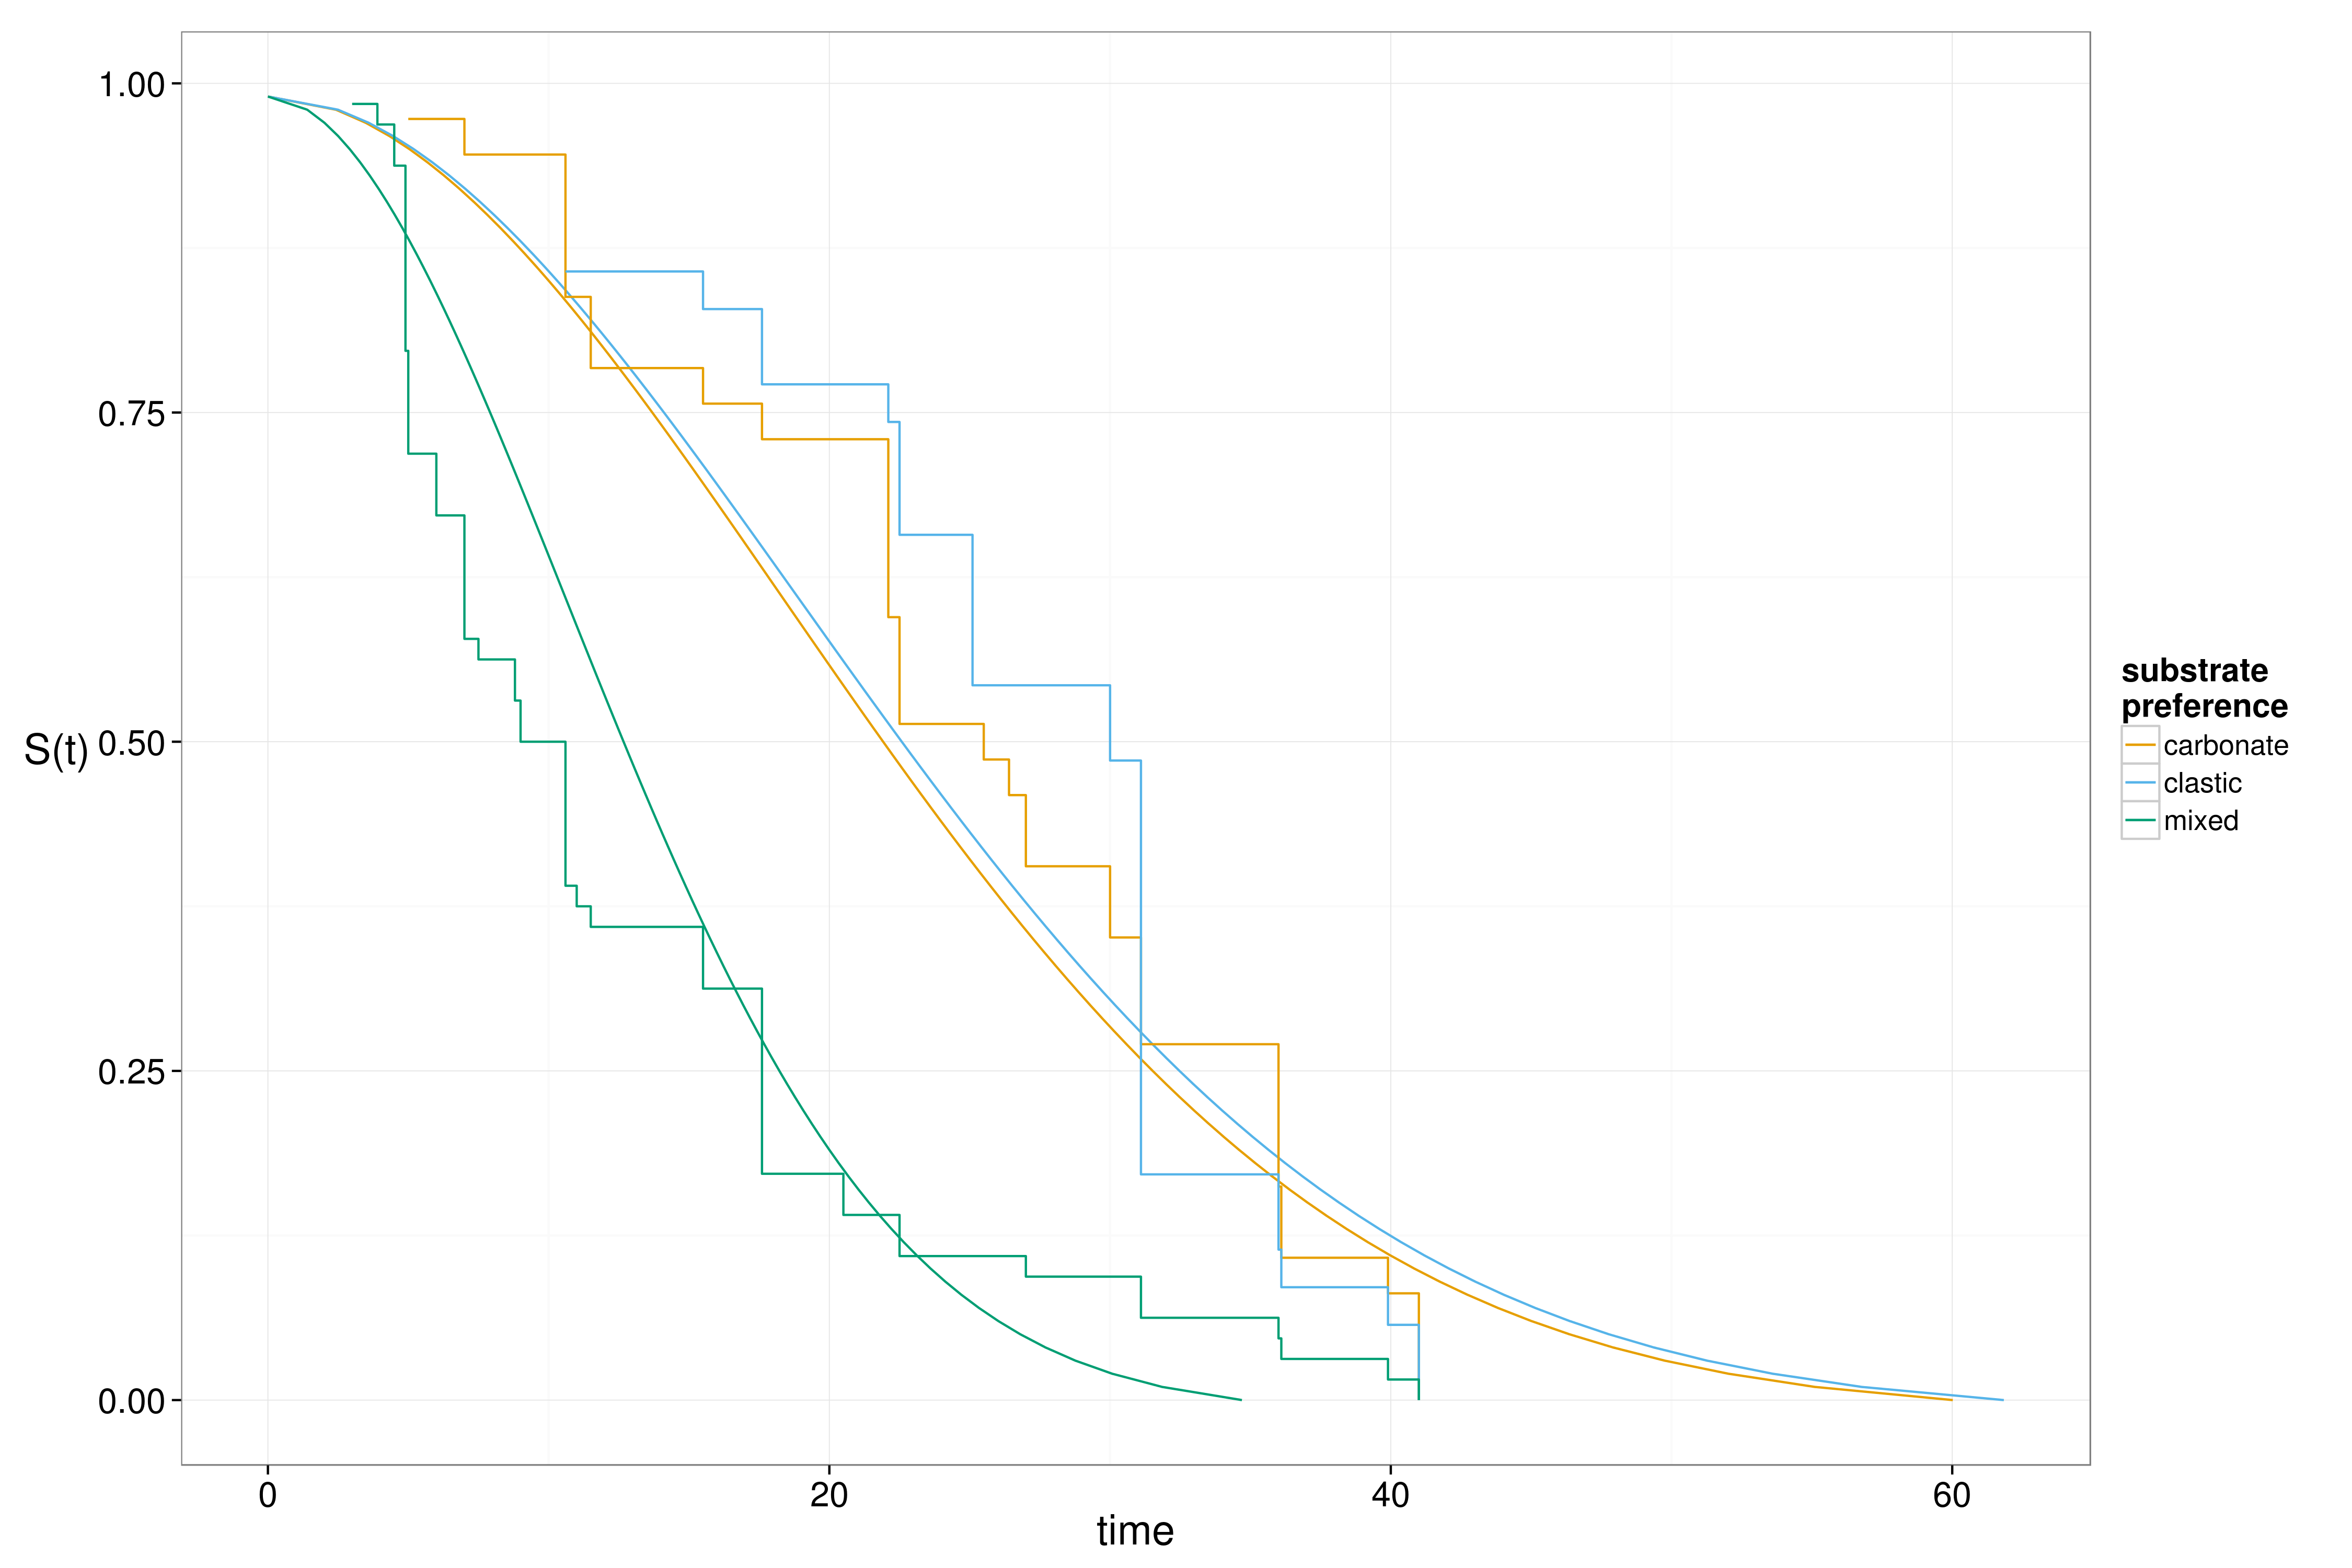
\includegraphics[height = 0.4\textheight, keepaspectratio = true]{figure/aff}
      \label{subfig:aff_surv}
    \end{subfigure}
    \begin{subfigure}[b]{0.5\textwidth}
      \caption{}
      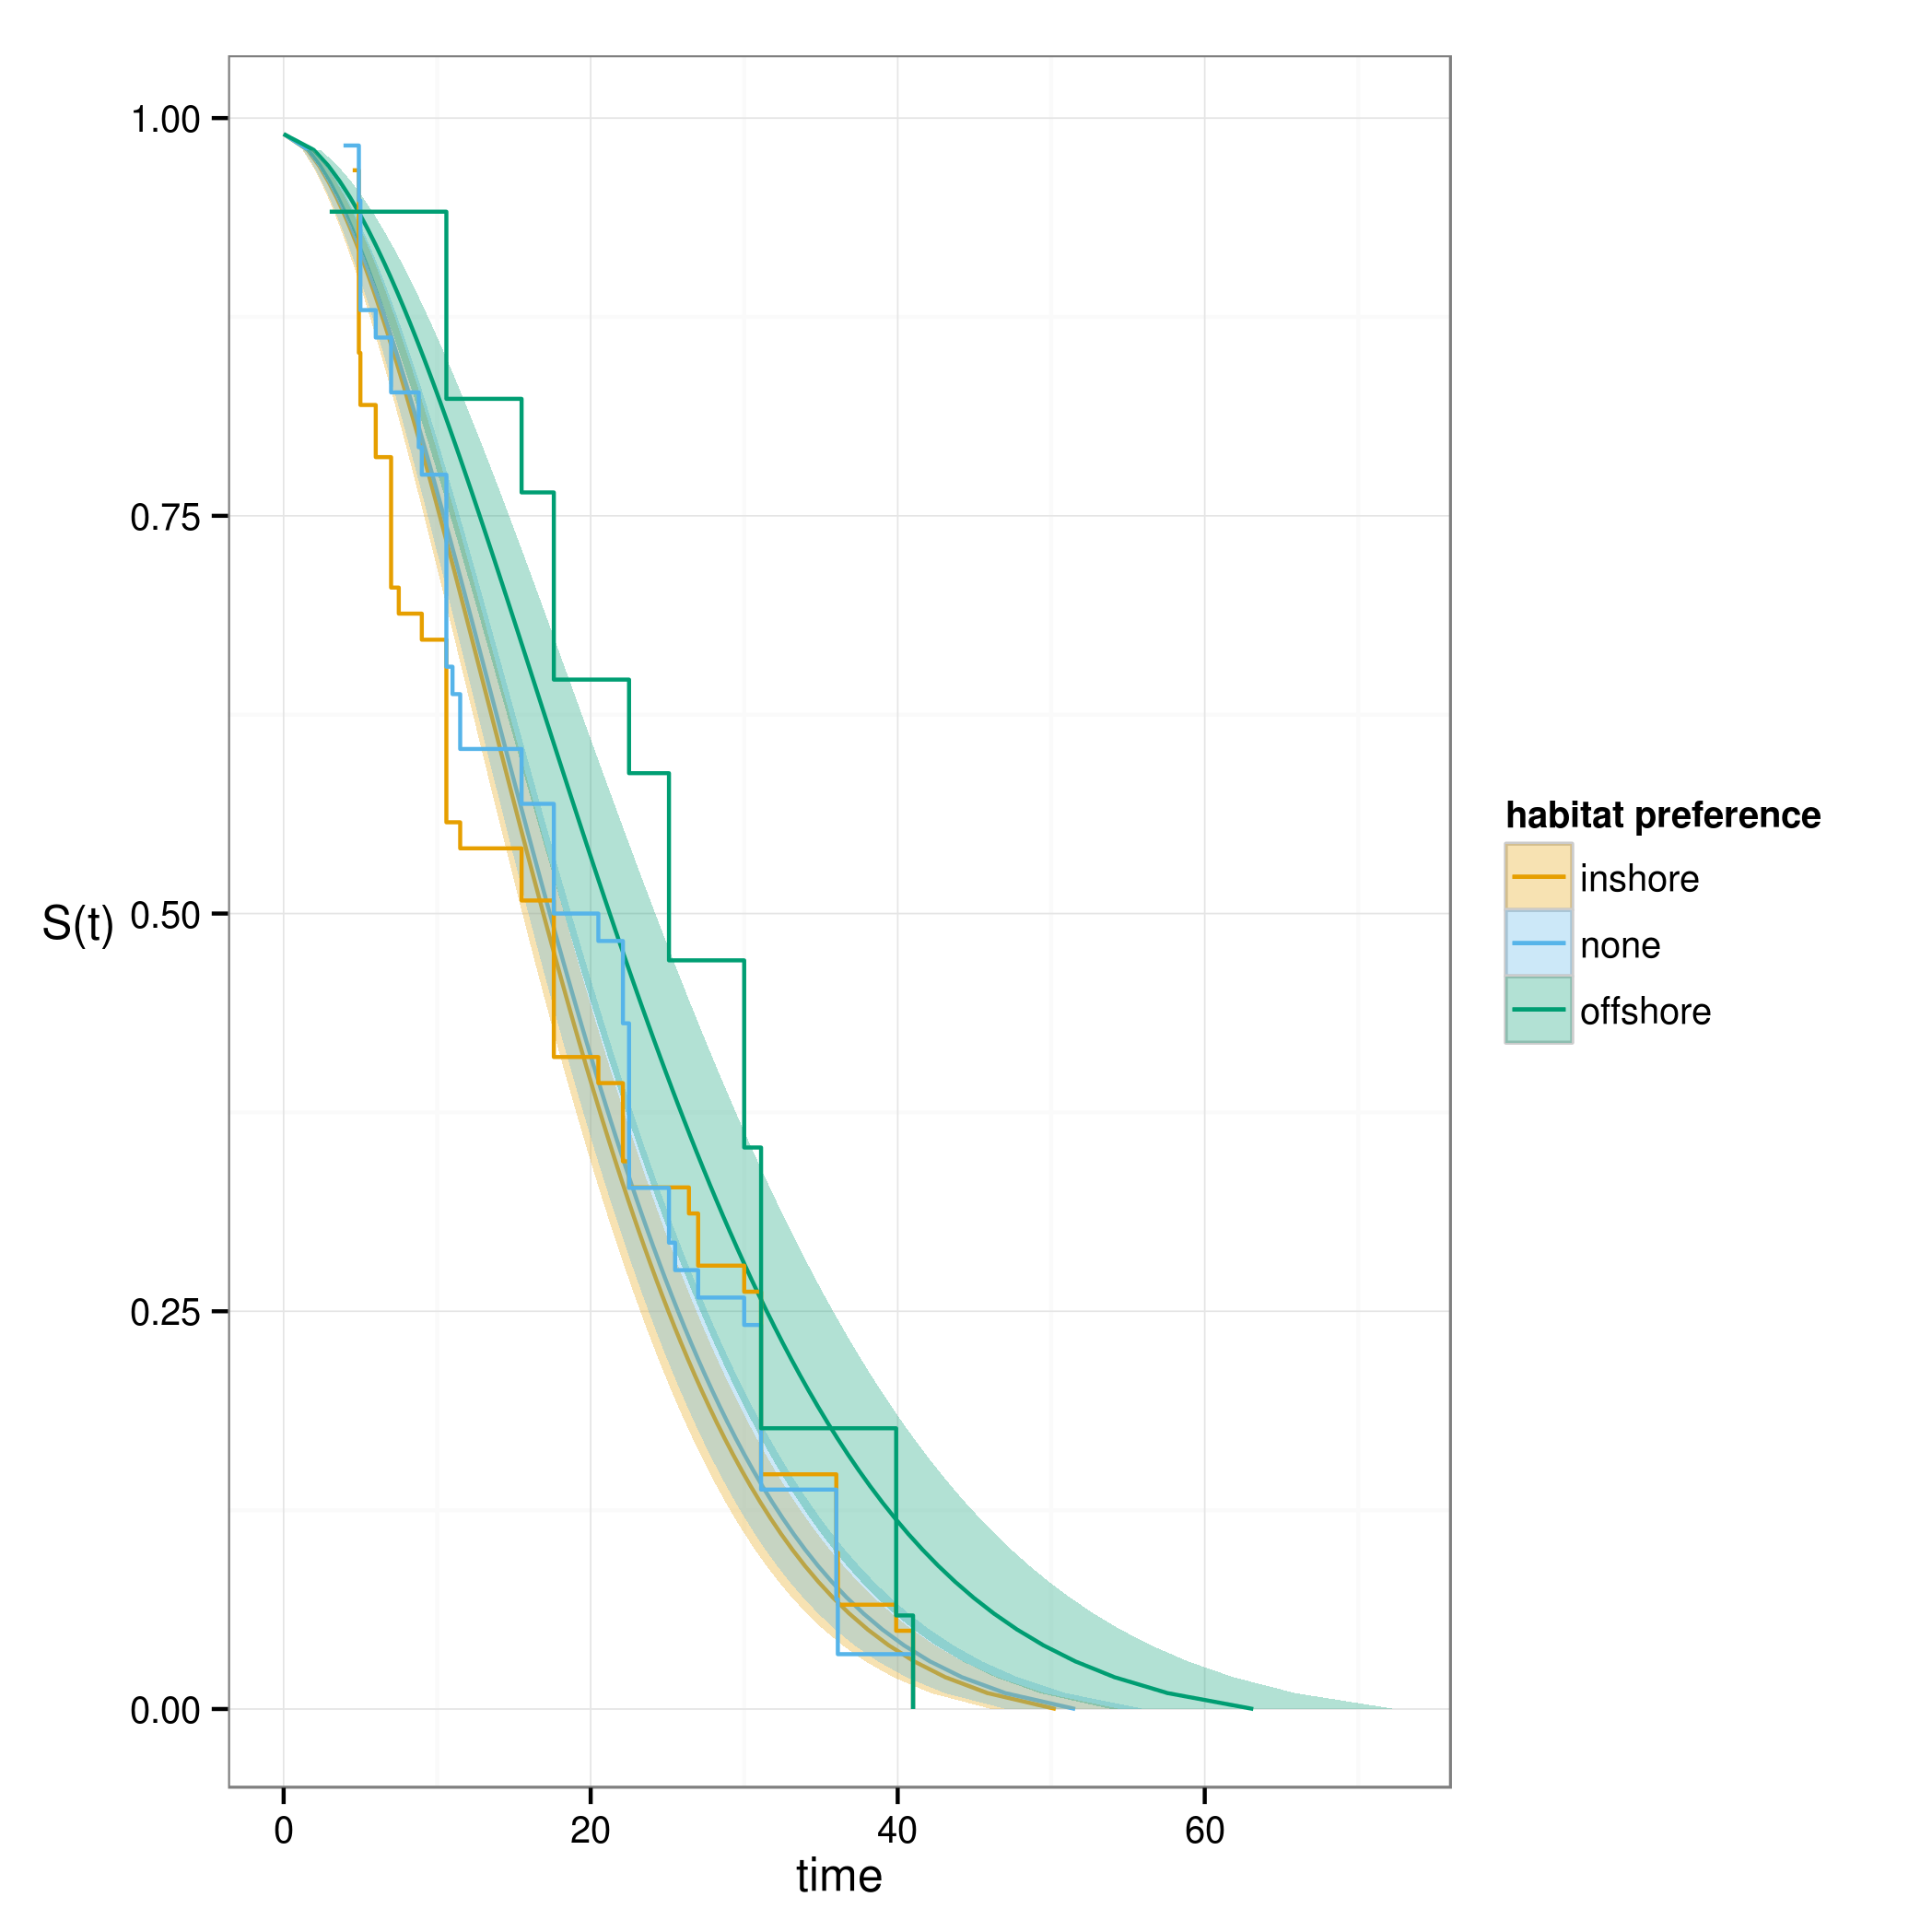
\includegraphics[height = 0.4\textheight, keepaspectratio = true]{figure/env}
      \label{subfig:env_surv}
    \end{subfigure}
%  \end{center}
    \caption{Survivorship curves of Australasian Permian brachiopod genera based on substrate affinity (\subref{subfig:aff_surv}) and habitat preference (\subref{subfig:env_surv}). The three stepwise functions are nonparametric Kaplan--Meier survival curves for each of the three substrate affinities. The three smooth lines are the predicted survivorship probabilities for taxon of the given age from the parametric model of generic survivorship and illustrated standard errors of the prediction.}
  \label{fig:brach_surv}
\end{figure}

The shape parameter (\(k\)) of the AICc best model (Fig. \ref{subfig:aff_surv}) is estimated to be approximately 1.9. As described above, values of \(k\) greater than 1 indicate that failure (extinction) rate is accelerating with respect to taxon age, which may mean that an age-independent extinction rate is inappropriate when modeling generic level diversification in brachiopods.

For brachiopods split but substrate affinity (Fig. \ref{subfig:aff_surv}), survival probabilities are higher in both carbonate and clastic lowest in taxa with mixed durations. Visual inspection of the estimated survival functions compared to the nonparametric Kaplan--Meier curves indicates that they are fairly good fits to the data. 

For brachiopods split by environmental affinity and survival modeled as a Weibull distribution is not a as good model of survival, with an approximate \(\Delta\)AICc of 33 between this model and the AICc best model. There is a great degree of deviance between the nonparametric Kaplan--Meier curves and the model predictions (Fig. \ref{subfig:env_surv}). Additionally, this model is not significantly different from the model with only an intercept (\(\chi^{2} = 2.41\), \(df = 2\), \(p = 0.3\)). This means, preliminarily, that habitat preference alone makes no difference in generic level extinction rate.

Further refinements to these models include modeling survival using other distributions of survival such as a log-normal distribution. Additionally the inclusion of affixing strategy as a predictor will increase the understanding of the biology underlying brachiopod generic survival based on organismal traits.


\section{Ecology, survivorship, and fitness in Cenozoic mammals}

\textit{Questions:} 
How do ecological traits related to range size affect mammalian taxon duration? Is any single trait the best predictor of mammalian survivorship, or do multiple traits together best model taxon duration? Is climate an important factor in modeling mammalian taxon duration?

\textit{Background and Predictions:} 
Three potential constituent traits of range size in mammals are dietary category, locomotor category, and body size \citep{Smith2004,Smith2008b,Damuth1981a,Damuth1979,Jernvall2004,Lyons2005,Lyons2010}. Each of these traits describes a different aspect of an organims relationship with the environment based on prey avaliabiilty, dispersal ability, or energetic cost.

Dietary cateogries are defined here as broad trophic categories that subsume further, more specific, classificaitons. The categories used here are carnivore, herbivore, omnivore, and insectivore. It should be noted that most prior analyses have not included insectivore as a category \citep{Jernvall2004,Price2012}. Similarly, locomotor categories are defined as combinations of more specific classifications and are broken into arboreal, ground dwelling, and scansorial/mixed. Both of these traits are constant at the specific level and thus there is no concerns about probability of assignment (see above).

Different dietary categories act as a limit on abundance because of the available environmental energy or resources in a location \citep{VanValen1989,Brown1987,Damuth1979,Silva1997,Janis2000}. Abundance is correlated with occupancy, or the number of unique localities at which a taxon is found \citep{Jernvall2002,Fortelius2002,Brown1984}. It follows then that limits imposed by environmental energy on abundance would then affect the (possible) range size of a taxon. Mammalian herbivores and carnivores have been found to have a greater diversification rate than omnivores \citep{Price2012}. This analysis was global in scope, and based purely on extant taxa in a comparative phylogenetic context. Diversification rate can increase via either an increase in origination relative to extinction or a decrease in extinction relative to origination. Which of these two processes is occurring is (currently) impossible to determine from a phylogeny of only extant organisms \citep{Rabosky2010a} which means that analysis of the fossil record is necessary to estimate which scenario is most likely to have occurred. 

Locomotor category describes the motility of a taxon and the plausibility of occurrence. Locomotor category also limits the dispersal ability of a taxon. For example, an obligate arboreal taxon can only occur in locations with a minimum of tree cover and can most likely only disperse to other environments with suitable tree cover. Dispersal ability is considered important in determining the extent of a taxon's geographic range \citep{Birand2012,Jablonski2006a,Gaston2009} and thus any trait that would limit the ability for an organism to disperse would most likely limit the range size of that organism. During the Cenozoic, between the Paleogene--Neogene, there was a shift from a predominatly closed environement to a predominately open environment. It is expected then that arboreal taxa during the Paleogene will have a greater expected duration than Neogene taxa, and the opposite will be true for ground dwelling taxa. In comparison, taxon duration in scansorial taxa is expected to remain relatively similar between the two time periods because it represents a mixed environmental preference that may be viable in either closed or open environments.

Similar to the dietary category, body size has an associated energetic cost in order to maintain homeostasis, which in turn necessitates enough of the appropriate supply of prey items. Because of this, it is expected that larger organisms have higher energetic costs and thus a greater range size in order to obtain necessary resources \citep{Damuth1979,Brown1987,Damuth1979,Lyons2010}. Depending on the continent, body size has been demonstrated to be related to extinction rate or not \citep{Tomiya2013,Liow2008}. By expanding to include a third continent, South America, I hope to elucidate how differences in taxonomic diversity at a continental level might affect body size mediated extinction rate. Additionally, I will be modeling body size as a continuous instead of binary variable.


\textit{Proposed research:}
To analyze differential mammalian survival, I propose a survival analysis approach similar to that described above for Permian brachiopods. Because dietary category and locomotor category are constant at the species level, they will be modeled as time-independent covariates of survival. While a species average body size may evolve over time, the resolution of the fossil record does not permit this for all taxa observed during the Cenozoic. Instead, following previous work, average body size will be considered constant with respect to time and will also be modeled as time-independent covariate. The climate proxy \(\delta O^{18}\) oxygen curve \citep{Zachos2008} will be modeled as an ancillary time-dependent covariate. Also, constant versus time varying extinction rate will be estimated using different fundamental hazard models by comparing the fit of survival to various probability distributions.

While many analyses of survivorship, such as the one described above for Permian brachiopods, are done using generic data \citep{Tomiya2013,Liow2008,Harnik2013}, there are potential biases in accurately modeling specific level processes using generic level data \citep{Raup1975,Sepkoski1975,Simpson2006,Raup1991a,VanValen1979}. Anagenesis, hierarchical selection, and taxa that did not go extinct in the time frame of interest may all bias estimation of the best model of survival \citep{Raup1975,VanValen1979,Simpson2006,Raup1991a}. Interestingly, the effect of incomplete sampling on estimation of survivorship curves appears rather minimal and uniform \citep{Sepkoski1975}. The problems involving taxa that did not go extinct have mostly been dealt with following advances in modeling right-censored and interval data \citep{Kleinbaum2005}.

In order to asses potential specific versus generic effects, I will estimate the difference between specific and generic mammalian survivorship models. Using an approach based on previous work to estimate specific origination and extinction rates from generic level survival curves \citep{Foote1988}, or a variant there of, I will measure the deviance between extinction rate estimated from the specific survivorship and the specific level extinction rates estimated from the analysis of the generic survivorship data. 

Additionally, in order to understand the effects of anagenesis and sampling on estimation of models of survival, I also propose a simulation study where these two properties are varied and the underlying survival functions are estimated. Because phylogenies are frequently simulated as a time-homogeneous birth-death process, this will be the model used to simulate the phylogenies underlying diversification. The is expected that for a time-homogeneous birth-death process, survival will be distributed exponentially because it will have an taxon age independent rate parameter (\(\lambda\)). While sampling has been found to have minimal effect on paleontological survival analysis assuming sampling is homogeneous across taxa \citep{Sepkoski1975}, the affect of anagenesis is unknown. 

Mammalian occurrence data will be collected through a combination of the PBDB, Neogene Old World Database (NOW; \url{http://www.helsink.fi/science/now/}), and museum collections. North American fossil mammal data is very well represented and vetted in the PBDB because of the extensive work of Alroy \citep{Alroy1996a,Alroy1998,Alroy2000g}. European fossil mammal data is also well represented between the PBDB and NOW. South American fossil mammal data is available through the PBDB, but is not particularly well vetted and has poor overall coverage. Because of this, South American fossil mammal data will be gathered via various museums such as the Field Museum of Natural History and the American Museum of Natural History as well as published occurrence compilations. With the South American taxa, taxonomy and sampling may not be as well resolved as for North and South America and it may be necessary to restrict analysis to the most taxonomically resolved and sampled groups such as Notoungulata, Marsupials, Carnivora, and Primates.


\section{Dynamics of community connectedness in Cenozoic mammals}

\textit{Questions:} 
How does the relationship between endemic and cosmopolitan taxa in average community composition change over time? Is there a single global pattern, or do different continents have different patterns? Do patterns differ between ecological categories? Is global climate change an important predictor of these patterns?

\textit{Background and Predictions:}
% move and heavilty revise this section to better reflect hypotheses and predictions as opposed to just listing each region. what are the differences I expect to witness?
Community connectedness is the degree to which localities are composed of endemic versus cosmopolitan taxa, and how similar this ratio is between all localities. How community composition changes over time and in relation to organismal traits as well as a changing environment is extremely important for understanding how trophic structure changes or is maintained as well as determining the relative importance of global, regional, or local processes. 

Community connectedness is measured here as four different summary statistics: average relative number of endemic taxa per locality, average relative locality occupancy per taxon, biogeographic connectedness, and code length \citep{Sidor2013}. These summary statistics describe on average how unique each locality is compared to all others during a time period, on average how endemic each taxon is relative to all taxon during a time period, how even taxa are distributed amongst localities during a time period, and the degree of biogeographic provinciality during a time period. The analysis of these summary statistics between and within different regions across the globe allows for the expected relative importance of global versus regional versus local processes and how these might change over time to be estimated.

In addition to regional community connectedness, the dynamics of taxa within various ecological categories is important to understanding whether different adaptive zones may be more affected by global, regional, or local processes. As described above, two important traits for potentially determining range size in mammals which are constant at the specific level are dietary category and locomotor category. 

During the Cenozoic there was a global shift from closed, forested habitat to open, savanna-like habitat. Importantly, the timing of this environmental shift was different between continents \citep{Stromberg2005,Stromberg2013}, so the patterns of community connectedness may not be globally uniform and could reflect regional differences. It is expected, then, that there would have been a relative increase in endemism and provincially accompanied by a decrease in biogeographic connectedness and occupancy in arboreal taxa over time. In contrast, the opposite is expected for terrestrial taxa. These expectations are because forested environments would likely have become increasingly patchily distributed, particularly during the Neogene compared to the Paleogene.

With regards to dietary category that occupancy will increase for herbivorous taxa, while increasing or remaining constant in carnivores, and remaining relatively constant or random for omnivores. These different predictions for each of the dietary categories is based on the differences in resilience and relationship with primary productivity, with herbivores being more resilient than carnivores and omnivores being random in their resilience \citep{Jernvall2004}. % EXPAND

An additional global trend during the Cenozoic was the shift from a ``hot house'' environment with no polar ice caps to an ``ice house'' environment with polar ice caps \citep{Zachos2008,Zachos2001}. This transition was known to have caused major shifts in the global climatic envelopes and the reorganization of communities along with it \citep{Janis1993a,Fortelius2002,Blois2009,Alroy2000g,Figueirido2012}. For mammalian community connectedness there are two possible scenarios. First, it could be possible that while the environment was shifting, lineages may have adapted in place and overall trophic structure and community connectedness would remained relatively constant through time, as observed during the Neogene of Europe \citep{Jernvall2004}. Alternatively, species may have shifted ranges and changed the average set of taxa present at a locality which would be associated with changes in trophic structure as well as community connectedness.

At a regional scale, community connectedness in North America is expected to follow the global predictions described above. This is because of the vast amount of prior work on the North American mammal fossil record \citep{Alroy2000g,Alroy1996a,Alroy1998,Barnosky2001a,Simpson1944,Simpson1953,Badgley2013,Blois2009,Figueirido2012,Gunnell1995,Hadly2001}. However, the effects of climate change on North American community connectedness remain unresolved and controversial \citep{Alroy2000g,Blois2009,Figueirido2012,Barnosky2001a}. 

The European mammalian fossil record is also well studied though research has focused primarily on faunal dynamics in the Neogene \citep{Jernvall2002,Jernvall2004,Liow2008,Raia2006,Raia2005,Raia2011c}. An important aspect about the European record is that during the Neogene there was little shift in relative dietary category abundance \citep{Jernvall2004} while the patterns within herbivores (browse--graze transition) were mostly driven by abundant, cosmopolitan taxa \citep{Jernvall2002}. It is predicted then that herbivores will demonstrate the same patterns of community connectedness as Europe as a whole, while omnivores and carnivores will be different from that of herbivores and may demonstrate random or constant patterns of community connectedness through time.

The biogeographic pattens of Cenozoic South American mammalian fauna are comparatively less studied than that of North American and Europe. Instead, cross--continental dynamics during the Neogene between North and South America are much more studied \citep{Marshall1982}. The South American mammalian faunal record reflects two distinct biotic provinces between the North and the South \citep{Macfadden1997,Macfadden2006,Flynn1998a,Patterson1968}. Because of this, the South American record is expected to have a different pattern of community connectedness than either North America or Europe. Also, there is an expected dramatic increase occupancy in land-dwelling herbivores relative to arboreal and scansorial taxa related to the aridification of high--latitude South America. % improve this a lot following Dave Polly's comments


\textit{Proposed research:}
Using methods first proposed by \citet{Sidor2013} and \citet{Vilhena2013}, I propose to construct bipartite biogeographic networks between taxa and localities. Here taxa are defined as species and localities are defined as 2x2 grid cells of an equal-area map projection. Networks will be made for every 2 million year bin of the Cenozoic. This bin width is chosen to have minimum two localities be present in every bin. Additionally, networks will be constructed for each dietary and locomotor category. Previous studies of mammalian occurrence patters have restricted analysis to major orders, such as Primates and Artiodactyls, in order to account for apparent sampling and taxonomic biases. Here, analysis will be done using all available taxa and with a restricted sample of just major orders in order to observe any differences in community connectedness.

Community connectedness will be measured using the four summary statistics described above. Average relative number of endemics is defined as 
%\begin{equation}
\(
  E = \frac{\sum_{i = 1}^{L} \frac{u_{i}}{n_{i}}}{L}
\)
%  \label{eq:end}
%\end{equation}
where \(L\) is as the number of localities, \(u\) is the number of taxa unique to a locality, and \(n\) is the number of taxa present at a locality. This is a measure of how unique localities are. Average relative occupancy is the number of localities where a taxon is, on average, found and is defined as 
%\begin{equation}
\(
  Occ = \frac{\sum_{i = 1}^{N} \frac{l_{i}}{L}}{N}
\)
%  \label{eq:occ}
%\end{equation}
where \(N\) is as the number of taxa present in the biogeographic network and \(l\) is the number of localities a taxon occurred in. Biogeographic connectedness is a measurement of the shared taxa between localities and is defined as 
%\begin{equation}
\(
  BC = \frac{O - N}{LN - N}
\)
%  \label{eq:bc}
%\end{equation}
where \(O\) is the total number of taxonomic occurrences. \(BC\) ranges from 0 to 1, with 0 meaning that each locality completely disconnected from all other localities and 1 indicating all that taxa shared between all localities. Importantly, \(BC\) is infinite when there is only one locality.

Code length is a measurement of the compressibility and information flow of a graph and is estimated via the map equation \citep{Rosvall2008,Rosvall2010b}. The logic of the map equation is that a good map compresses reality into a few simple symbols. This means we want to compress each section of a graph into individual single symbol. A network with a low code length can be compressed into more distinct subunits/provinces compared to a network than a large code length. In the case of measuring community connectedness, a low code length means greater provinciality than a high code length \citep{Sidor2013}. % monte carlo simulations to show what code length actually measures? Rewire with the same summary stats? Simulate bipartite networks? Deal with Dave Polly's comments.

Phylogenetic similarity between localities may play an important role in community structuring \citep{Webb2002} such as closely related taxa being ``repulsed'' due to similarity in niche or ``clumped'' because of inability to disperse. As a preliminary approach, for every pairwise combination of localities during a time period an informal phylogeny will be constructed for the pool of all taxa present in both localities. This informal phylogeny will be based solely on available taxonomic information such as order, family, and genus assignments. The average patristic distance between all taxa will then be estimated. The average of all pairwise comparisons can then be used in partial correlations and modeling questions for understanding what best explain patterns of community connectedness.

The next step is to compare patterns of community connectedness both within and between regions in order to understand if there is a single global trend or if regional processes dominate as well as comparisons of the different dietary and locomotor categories for similarity within and between traits and regions. The approach and methodology to accomplish this analysis is currently under development. 

The data necessary to complete this study will be the same as for the above analysis of mammalian survival.

\textit{Preliminary results}
Preliminary results of the community connectedness patterns of both North America and Europe based on PBDB data are presented here (Fig. \ref{fig:mam_tot}). Both regions have qualitatively very different patterns of community connectedness, primarily during the Paleogene. Almost all four of the summary statistics are extremely volatile over the Cenozoic, especially for the European record. However, there some interesting qualitative patterns present.

\begin{figure}[ht]
  \begin{center}
    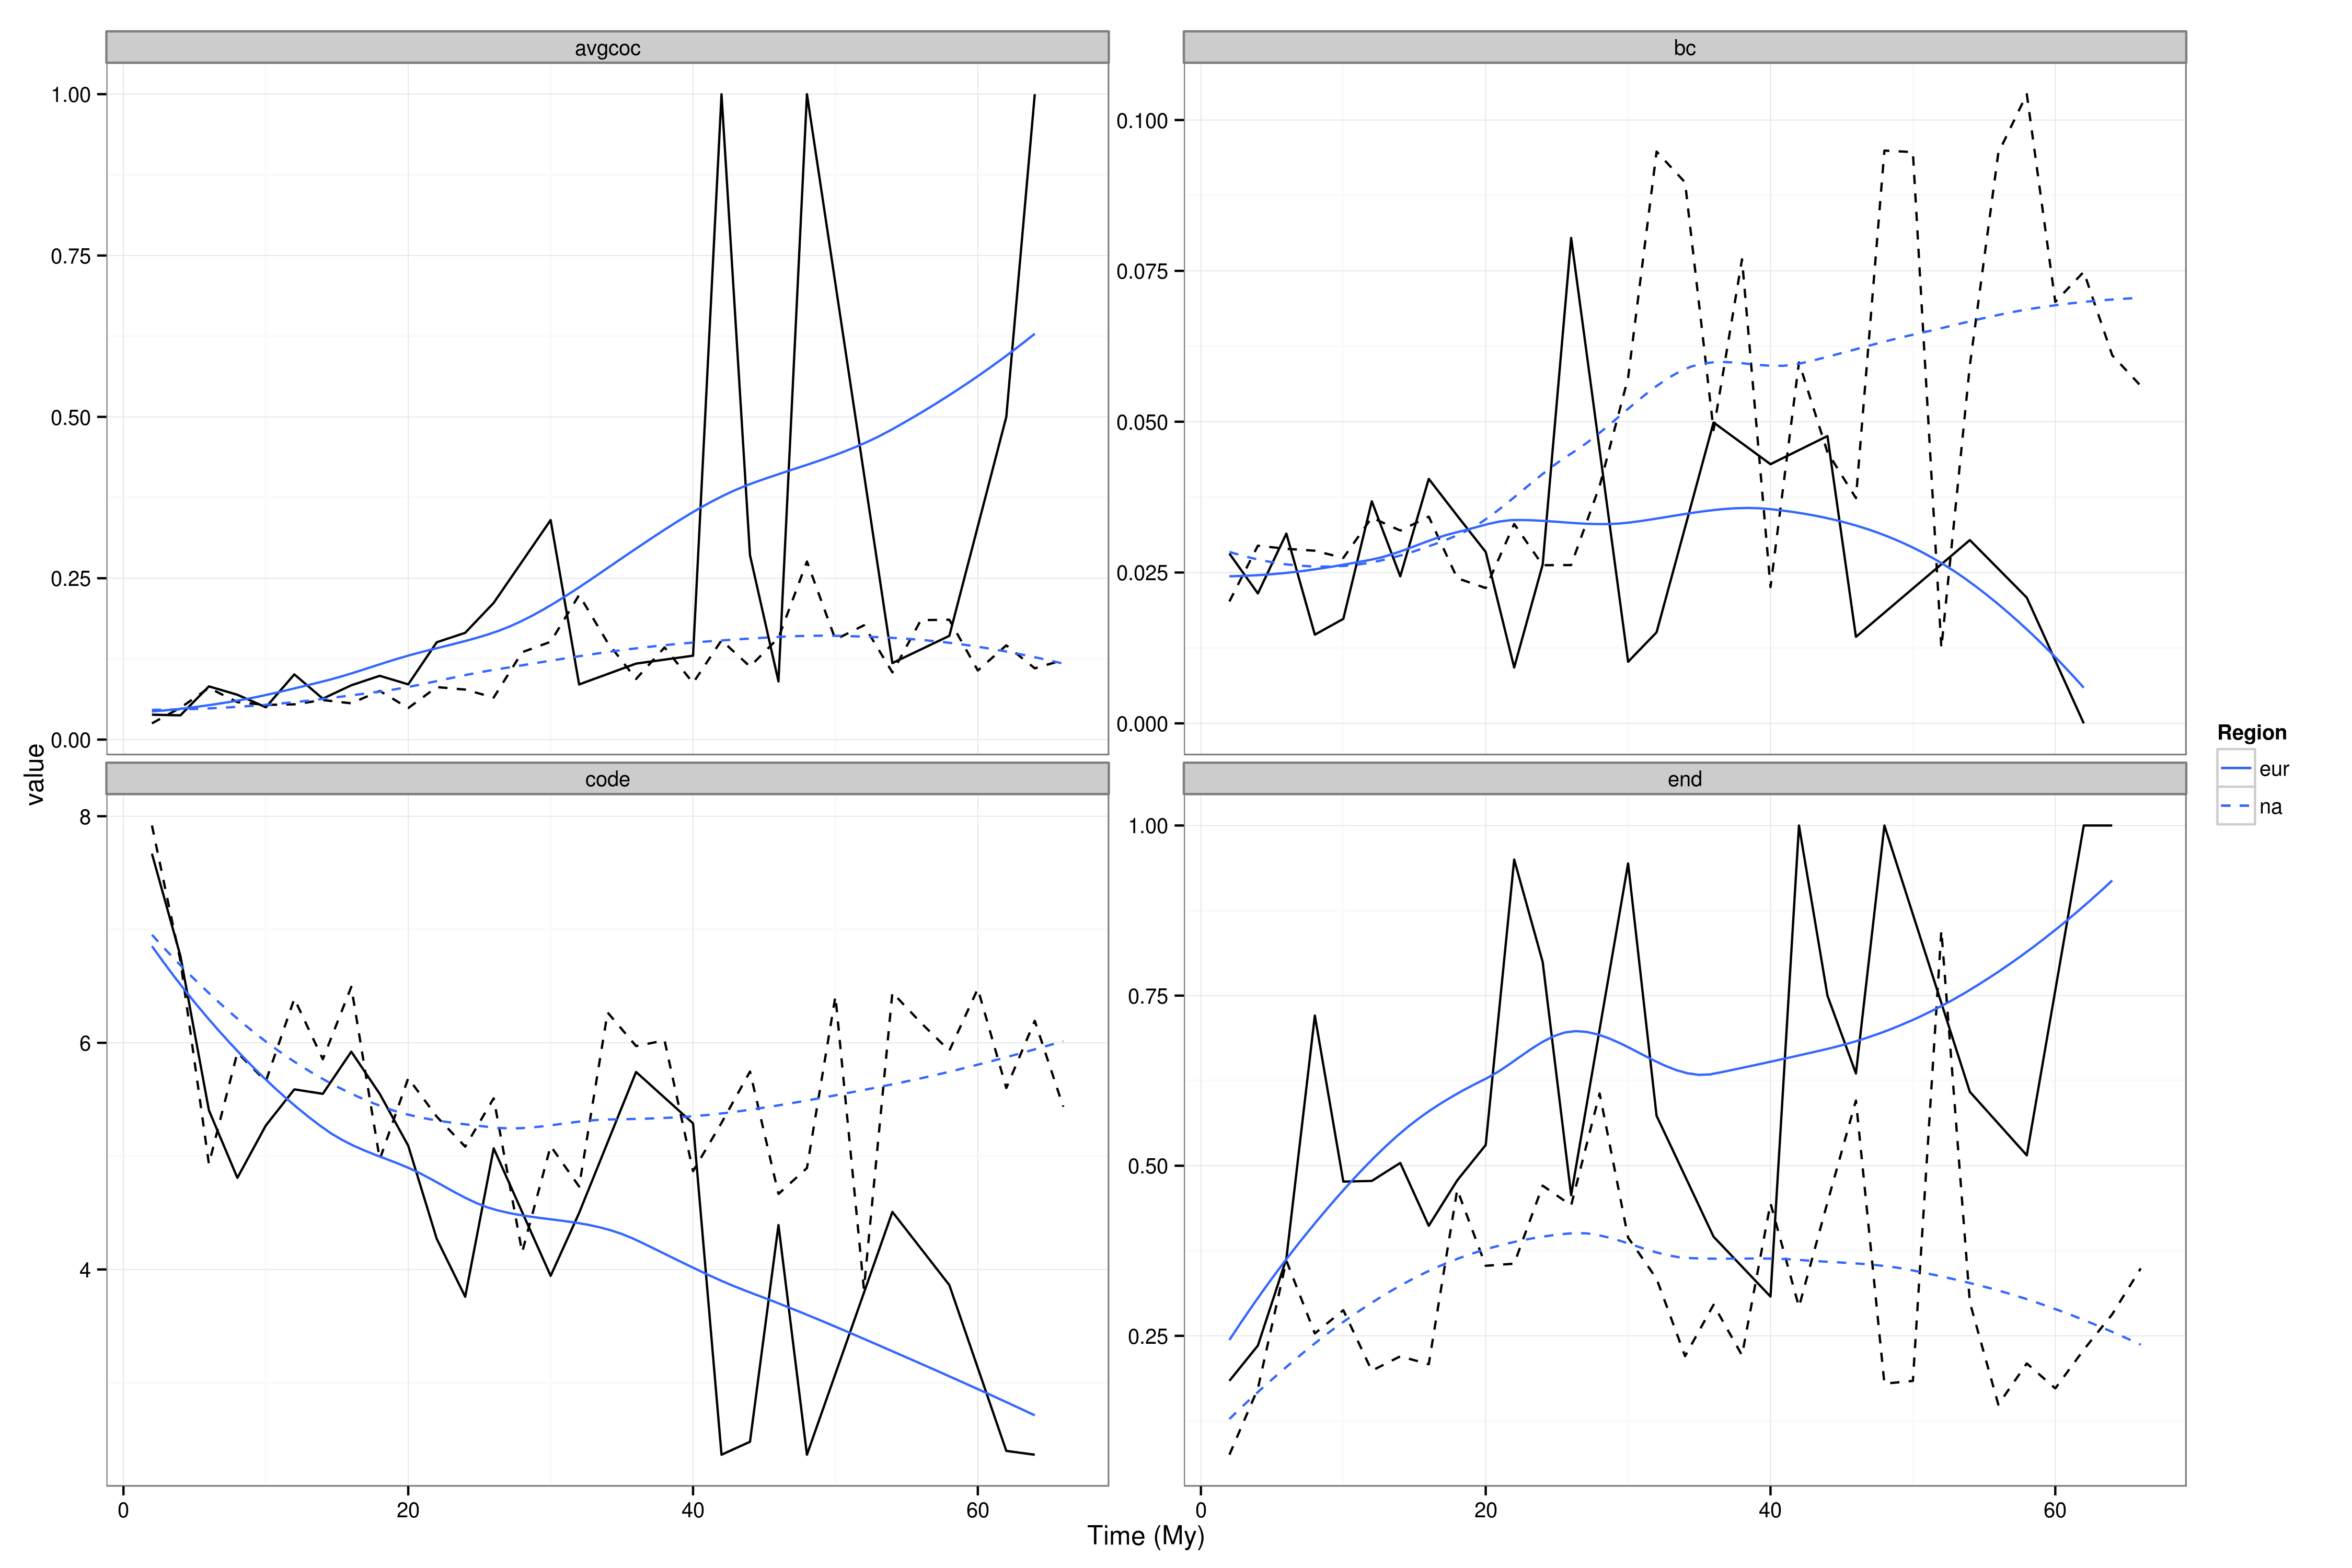
\includegraphics[height = 0.4\textheight, keepaspectratio = true]{figure/gen_bin}
  \end{center}
  \caption{Biogeographic network summary statistics for mammalian communities in North America (dashed line) and Europe (solid line). The summary statistics are, clockwise from top left: average relative occupancy (avgcoc), biogeographic connectedness (bc), average relative number of endemics (end), code length (code). Blue lines are generalized additive model smooths and are presented to illustrate the over all pattern of the two regions.} 
  \label{fig:mam_tot}
\end{figure}

While average relative occupancy remains relatively stationary for North America, there is a qualitative decrease in average relative occupancy in Europe until approximately the start of the Neogene (approximately 23 My). Average relative occupancy is a measure of how cosmopolitan any individual taxon is and the qualitative decrease in average relative occupancy in Europe over the entire Cenozoic indicates that the average taxon is becoming generally less cosmopolitan over time. In contrast, average relative occupancy in North America is qualitatively stationary over the entire Cenozoic and almost always lower than that observed for the European record. This means that, on average, North American taxa are present in very few localities at any given point in time.

Biogeographic connectedness is a measure of shared taxa between all localities, and higher values mean that more shared taxa then when there are lower values. Biogeographic connectedness of North American mammalian communities qualitatively decreases over the early Cenozoic until approximately the start of the Neogene. In Europe there is a qualitative rise in biogeographic connectedness in the first few million years of the Cenozoic, but afterwards remains relatively stationary. This may indicate that the average proportion of shared taxa remained qualitatively stationary. In comparison, North American remains stationary with a greater amount of shared taxa than Europe for the first half of the Cenozoic followed by a decrease and another plateau at the end of the Cenozoic.

In Europe, there is a over all qualitative decrease in average relative number of endemic taxa. North America, in contrast, has a qualitatively constant average relative number of endemics over the Cenozoic with a slight decrease in the Neogene. As discussed above, average relative number of endemics is a measure of relative uniqueness of localities. Qualitatively, North America retained approximately the same amount of site uniqueness through out the Cenozoic. In comparison, the pattern of the European record shows a qualitativly nonmonotonic decrease in locality uniqueness because of the decrease in average relative number of endemics.

The code length of European biogeographic networks increases qualitatively over the entire Cenozoic, while code length of North American networks remains relatively constant until the Neogene when there is a qualitative increase. Code length acts as a measure of general provinciality, with a high code length indicating little provincially between localities. Initial interpretation of these results indicates that North America maintains a stationary degree of provinciality while Europe has a qualitatively decreasing degree of provinciality. 


\section{Summary of proposed research}
One of the most important questions in (paleo)biology is why do certain species go extinct while others do not? Elucidating what interactions, or traits governing interactions, are important when estimating survival is then extremely important and a fundamental concern of evolutionary paleoecology. While the species level property of range size is continually found to be an extremely vital for both origination and extinction \citep{Roy2009c,Foote2013,Jablonski2003,Jablonski1987,Harnik2013}, how candidate constituent lower level traits are necessary to ``form'' this emergent property remains more nebulous and is instead frequently framed as which traits in addition to range size \citep{Foote2013,Harnik2011,Nurnberg2013a}. If the favored models of survival include the additive or interactive effects of multiple organismal traits then this is possibly the signature of emergence, particularly in the case of interaction. Related to this is the ``law'' that extinction risk within an adaptive zone is taxon age independent \citep{VanValen1973}. Here I analyze two biologically different clades in order to understand patterns of survival and expectations of whether global, regional, or local process should dominate. By comparing the patterns of survival in brachiopods and mammals it should be possible to determine when different variables matter to survival and when they do not and potentially how they matter.


\clearpage
\section{Timeline}

Spring/Summer 2014
\begin{itemize}
  \item Evolution Meeting: preliminary brachiopod survival results
  \item South American fossil mammal data from Field Museum of Natural History collections
\end{itemize}

Fall 2014/Winter 2015
\begin{itemize}
  \item GSA: survivorship simulation for anagenesis and sampling
  \item Doctoral Dissertation Improvement Grant
\end{itemize}

Spring/Summer 2015
\begin{itemize}
  \item Evolution Meeting: mammalian survivorship analysis for North America and Europe
  \item South American fossil mammal data from American Museum of Natural History collections
  \item write and submit survivorship simulation paper
\end{itemize}

Fall 2015/Winter 2016
\begin{itemize}
  \item SVP or GSA: mammalian biogeographic connectedness
  \item write and submit mammal connectedness paper
\end{itemize}

Spring/Summer 2016
\begin{itemize}
  \item Evolution Meeting: brachiopod survival analysis results
  \item write and submit brachiopod survival paper
\end{itemize}

Fall 2016/Winter 2017
\begin{itemize}
  \item SVP or GSA: mammalian survivorship analysis
  \item write and submit mammal survival paper
\end{itemize}

Spring/Summer 2017
\begin{itemize}
  \item Evolution Meeting
  \item write and submit review/philosophy paper
  \item \textbf{Defend}
\end{itemize}



\clearpage
\bibliographystyle{abbrvnat}
\bibliography{proposal}

\end{document}
